\subsection{Simulated Annealing}

Simulated annealing is a stochastic algorithm that attempts to find the global optimum of an objective function $f(x)$. The method is inspired by statistical physics, in particular the Boltzmann distribution that specifies the probability of being in a particular state $x$:
\begin{equation}
    p(x) \propto \exp\{-f(x)/T\}
\end{equation}
where $f(x)$ is the energy of the system and $T$ is the temperature. As the temperature approaches zero, the system spends more and more time in its minimum energy (most probable) state. As the temperature decreases, the largest peaks become larger and the smallest peaks dissappear. By cooling slowly enough, it is possible to track the largest peak and therefore find the global optimum.\\

Simulated annealing is closely related to the Metropolis-Hastings algorithm for generating samples from a probability distribution. At each step of the algorithm, we sample a new state according to a proposal distribution $x^{\prime} \sim q(\dot|x_k)$, such as a random walk proposal:
\begin{equation}
    x^{\prime} = x_k + \epsilon_k, ~~~ \mathrm{where}~ \epsilon_k \sim N(0,\Sigma)
\end{equation}
Having proposed a new state, we compute $\alpha$ as in Algorithm \ref{alg:sim_annealing}.
\begin{algorithm}
\caption{Simulated Annealing}
\label{alg:sim_annealing}
\begin{algorithmic}[1]
\STATE $\alpha = \exp\{(f(x)-f(x^{\prime}))/T\}$
\STATE $r = \min(1,\alpha)$
\STATE $u \sim \mathrm{Unif}(0,1)$
\STATE if $u < r$ 
\STATE ~~~ $x_{k+1} = x^{\prime}$
\STATE else
\STATE ~~~ $x_{k+1} = x_k$
\STATE end if  
\end{algorithmic}
\end{algorithm}
Thus, if a new state has lower energy (higher probability), we will definitely accept it but if it has higher energy (lower probability), we might still accept it depending on the temperature. Therefore, the algorithm allows downhill moves in probability space but less frequently as the temperature drops. In practice it is common to use an exponential cooling schedule: $T_k = T_0 C^{k}$, where $T_0 \sim 1$ is the initial temperature and $C \sim 0.8$ is the cooling rate. Cooling too quickly can result in getting stuck in local optima, while cooling too slowly wastes time. The optimum cooling schedule is difficult to determine.    

\begin{figure}[tbhp]
    \centering
    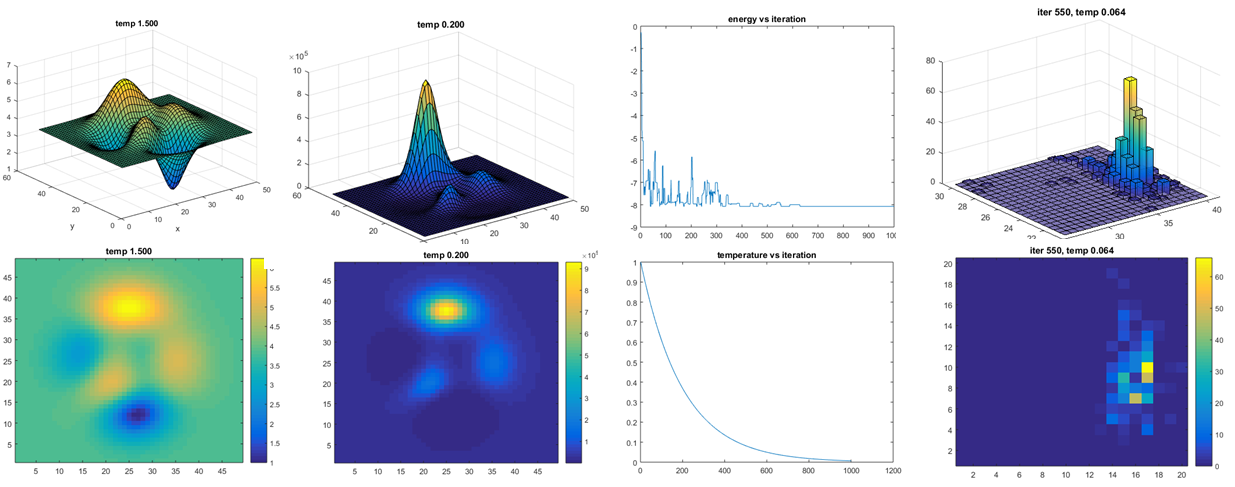
\includegraphics[width=0.9\textwidth, trim={10 10 10 10}]{figures/sim_annealing_merged.png}
    \caption{Simulated Annealing}
    \label{fig:sim_annealing_merged}
\end{figure}

Figure \ref{fig:sim_annealing_merged} shows the objective $f(x)$ at two different temperatures (left). The function appears more peaky when the temperature is lower. We can also see that the method stochastically reduces the energy over time for the given cooling schedule (middle). Finally a histogram of samples shows that most samples are concentrated near the global maximum (right).




